\documentclass[10pt]{beamer}
\usefonttheme{professionalfonts}
%\usetheme{CambridgeUS}
%
% Choose how your presentation looks.
%
% For more themes, color themes and font themes, see:
% http://deic.uab.es/~iblanes/beamer_gallery/index_by_theme.html
%
\mode<presentation>
{
  \usetheme{default}      % or try Darmstadt, Madrid, Warsaw, ...
  \usecolortheme{beaver} % or try albatross, beaver, crane, ...
  \usefonttheme{default}  % or try serif, structurebold, ...
  \setbeamertemplate{navigation symbols}{}
  \setbeamertemplate{caption}[numbered]
} 

\usepackage[english]{babel}
\usepackage[utf8x]{inputenc}
\usepackage{tikz}
\usepackage{pgfplots}
\usepackage{array}  % for table column M
\usepackage{makecell} % to break line within a cell
\usepackage{verbatim}
\usepackage{graphicx}
\usepackage{epstopdf}
\usepackage{amsfonts}
\usepackage{xcolor}
\usepackage{ifthen}
%\usepackage{mathtools}
\usepackage[makeroom]{cancel}
\usetikzlibrary{spy}
%\captionsetup{compatibility=false}
%\usepackage{dsfont}
\usepackage[absolute,overlay]{textpos}
\usetikzlibrary{calc, angles,quotes}
\usetikzlibrary{pgfplots.fillbetween, backgrounds}
\usetikzlibrary{positioning}
\usetikzlibrary{arrows}
\usetikzlibrary{pgfplots.groupplots}
\usetikzlibrary{arrows.meta}
\usetikzlibrary{plotmarks}
\usetikzlibrary{decorations.markings}
\usepgfplotslibrary{groupplots}
\pgfplotsset{compat=newest} 
%\pgfplotsset{plot coordinates/math parser=false}

\usepackage{hyperref}
\hypersetup{
    colorlinks=true,
    linkcolor=blue,
    filecolor=magenta,      
    urlcolor=cyan,
}

%
%\def\EXTERNALIZE{1}
%%% Page numbering
\usepackage{etoolbox} % necessary for excluding beamer-only frames from page numbering

\makeatletter
\pretocmd{\beamer@@@@frame}{\alt<#1>{}{\beamer@noframenumberingtrue}}{}{}
\makeatother

\addtobeamertemplate{navigation symbols}{}{%
	\usebeamerfont{footline}%
	\usebeamercolor[fg]{footline}%
	\hspace{1em}%
	\insertframenumber/\inserttotalframenumber
}
%%%

\definecolor{matlabcomment}{RGB}{34,139,34}

\pgfmathdeclarefunction{gauss}{1}{%
	\pgfmathparse{1/(sqrt(2*pi))*exp(-((#1)^2)/2)}%
}

\pgfmathdeclarefunction{laplacian}{2}{%
	\pgfmathparse{1/(#2*2)*exp(-(abs(x-#1))/(#2))}%
}

\pgfmathdeclarefunction{pretty_func}{1}{%
	\pgfmathparse{cos(deg(#1/2)) - sin(deg(#1)) + cos(deg(#1/2)-45) - sin(deg(#1/4)-154)}%
}

\pgfplotsset{
	dirac/.style={
		mark=triangle*,
		mark options={scale=2},
		ycomb,
		scatter,
		visualization depends on={y/abs(y)-1 \as \sign},
		scatter/@pre marker code/.code={\scope[rotate=90*\sign,yshift=-2pt]}
	}
}

\def\thickness{very thick}

\tikzset{
amark/.style 2 args={
	decoration={             
		markings, 
		mark=at position {0.5} with { 
			\arrow{stealth},
			\node[#2] {#1};
		}
	}, \thickness,
	postaction={decorate}
},
earlymark/.style 2 args={
	decoration={             
		markings, 
		mark=at position {0.25} with { 
			\arrow{stealth},
			\node[#2] {#1};
		}
	}, \thickness,
	postaction={decorate}
},
latemark/.style 2 args={
	decoration={             
		markings, 
		mark=at position {0.8} with { 
			\arrow{stealth},
			\node[#2] {#1};
		}
	}, \thickness,
	postaction={decorate}
},
zpath/.style={
	decoration={             
		markings, 
		mark=at position {0.5} with { 
			\arrow{stealth},
			\node[#1] {$z^{-1}$};
		}
	}, \thickness,
	postaction={decorate}
},
terminal/.style 2 args={draw,circle,inner sep=2pt,label={#1:#2}},
}


\tikzset{
	invisible/.style={opacity=0},
	visible on/.style={alt={#1{}{invisible}}},
	alt/.code args={<#1>#2#3}{%
		\alt<#1>{\pgfkeysalso{#2}}{\pgfkeysalso{#3}} % \pgfkeysalso doesn't change the path
	},
}

\newcommand\PlotSampledSpectrum[4]{%
	\def\fs{#2}%
	\def\fmax{#3}%
	\def\ros{#4}%
	\input{#1}%
}

\pgfmathdeclarefunction{invgauss}{2}{%
	\pgfmathparse{sqrt(-2*ln(#1))*cos(deg(2*pi*#2))}%
}

\tikzset{
	declare function={
		sinc(\x) = (and(\x!=0, 1) * (sin(deg(pi*\x))/(pi*\x)) +
		(and(\x==0, 1) * 1);
	}
}

\DeclareMathOperator{\E}{\mathbb{E}} % expectation

\newcolumntype{M}[1]{>{\centering\arraybackslash}m{#1}}

\definecolor{blue2}{RGB}{51, 105, 232}  
\definecolor{red2}{RGB}{213, 15, 37}  
\definecolor{green2}{RGB}{0, 153, 37}  
\definecolor{green3}{rgb}{0.1922, 0.6392, 0.3294}% 
\definecolor{yellow2}{RGB}{238, 178, 17} 
\definecolor{gray2}{RGB}{102, 102, 102}
\definecolor{orange2}{RGB}{230, 85, 13}

% Qualitative pallete set1 from www.ColorBrewer.org
\definecolor{Qred}{RGB}{228,26,28}
\definecolor{Qblue}{RGB}{55,126,184}
\definecolor{Qgreen}{RGB}{77,175,74}
\definecolor{Qpurple}{RGB}{152,78,163}
\definecolor{Qorange}{RGB}{255,127,0}
\definecolor{Qyellow}{RGB}{255,255,51}
\definecolor{Qbrown}{RGB}{166,86,40}
\definecolor{Qpink}{RGB}{247,129,191}
\definecolor{Qgray}{RGB}{153,153,153}

\newcommand\SimpleSys[4]{%
	\def\xin{#2}%
	\def\Hz{#3}%
	\def\yout{#4}
	\input{#1}%
} % some definitions

%% 
\title[EE 264]{Review and Conclusions}
\author{Jose Krause Perin}
\institute{Stanford University}
\date{August 17, 2017}

\begin{document}

\begin{frame}
  \titlepage
\end{frame}

%
\begin{frame}{Announcements}
\begin{itemize}
	\item End-quarter teaching evaluations are available on Axess
	\item Final exam logistics
	\begin{itemize} \normalsize
		\item You'll receive the final exam and accompanying files via email at the time you indicated in the sign up sheet.
		\item You have 24 hours to turn in your solutions on Canvas
		\item You may use any available references, but all the work must be done individually
		\item Do not communicate with others about the exam even after you have taken it
	\end{itemize}
\end{itemize}
\end{frame}

%
\begin{frame}{Outline}
	\tableofcontents
\end{frame}

%
\section{Review}
\subsection{Random processes}
\begin{frame}{Random processes}
\begin{itemize}
	\item We use random processes to model signals that cannot be easily described by simple equations
	\item A random process is wide-sense stationary (WSS) if its mean is constant and if its autocorrelation function is only a function of the time difference. 
	\item A random process is ergodic if its time averages are equal to its probability averages
	\item Autocorrelation functions must be real, even symmetric, and must have non-negative Fourier transform.
	\item The Fourier transform of the autocorrelation function is called the power spectrum density (PSD). The PSD has units of W/Hz or dBm/Hz.
	\item Random processes that have PSD constant over all frequencies are called white noise
	\begin{equation*}
		\Phi_{xx}(e^{j\omega}) = \sigma_x^2 \Longleftrightarrow \phi_{xx}[m] = \sigma_x^2\delta[m] \tag{white noise}
	\end{equation*}
\end{itemize}
\end{frame}

%
\begin{frame}{Random processes}
Effect of filtering random signals
\begin{center}
	\resizebox{0.7\linewidth}{!}{\def\layersep{3cm}
\def\dy{1.25}

\begin{tikzpicture}[draw=black!50, node distance=\layersep, font=\sffamily]
    \tikzstyle{node}=[circle,fill=black,minimum size=2pt,inner sep=0pt]
    \tikzstyle{block}=[draw=black,rectangle,fill=none,minimum width=3cm, minimum height=2cm, inner sep=0pt]
    \tikzstyle{annot} = []

	\node[node] (xc) {};
    \node[block, text width = 2.5cm, align= center, right of=xc] (DSP) {$h[n]\leftrightarrow H(e^{j\omega})$};
	\coordinate[right of=DSP] (yc) {};
		
    \path[->, >=stealth, shorten >= 0pt] (xc) edge (DSP);
    \path[->, >=stealth, shorten >= 0pt] (DSP) edge (yc);
    
    \node[below = 0.5mm of xc, text width=2.5cm, align=center] {Random signal \\ $x[n]$};	
    \node[below = 0.5mm of yc] {$y[n]$};
    
   	\node[node, below=2.5cm of xc] (phix) {};
   	\node[block, text width = 3cm, align= center, right of=phix] (DSP2) {$h[m]\ast h^*[-m] \leftrightarrow |H(e^{j\omega})|^2$};
   	\coordinate[right of=DSP2] (phiy) {};
   	
   	\path[->, >=stealth, shorten >= 0pt] (phix) edge (DSP2);
   	\path[->, >=stealth, shorten >= 0pt] (DSP2) edge (phiy);
   	
   	\node[below = 0.5mm of phix, text width=1.5cm, align=center] { $\phi_{xx}[m]$};	
   	\node[below = 0.5mm of phiy] {$\phi_{yy}[m]$};
\end{tikzpicture}}
\end{center}

\begin{itemize}
	\item The input autocorrelation function is \textit{filtered} by the LTI system defined by $h[n]\ast h^*[-n] \leftrightarrow |H(e^{j\omega})|^2$
	\item $c_{hh}[n] = h[n]\ast h^*[-n]$ is called the deterministic autocorrelation function.
	\item Average power after filter
	\begin{equation*}
		\sigma^2_y = \phi_{yy}[0] = \frac{1}{2\pi}\int_{-\pi}^{\pi} \phi_{yy}(e^{j\omega}) d\omega
	\end{equation*}
\end{itemize}
\end{frame}


\subsection{Sampling, reconstruction, and DT filtering}
\begin{frame}{Sampling, reconstruction, and DT filtering}
\begin{itemize}
	\item Sampling a continuous-time signal results in replicas of the spectrum at multiples of the sampling frequency $\Omega_s$ (or $2\pi$ of the normalized frequency $\omega$)
	\item A band-limited signal has highest frequency $\Omega_N$ ($X_c(j\Omega) = 0, |\Omega| > \Omega_N$)
	\item If a band-limited signal is oversampled ($\Omega_s > 2\Omega_N$) there'll be gaps between the spectrum replicas
	\item If the signal is undersampled ($\Omega_s < 2\Omega_N$) the spectrum replicas will overlap resulting in aliasing distortion
	\item We can perfectly reconstruct a signal from its samples, provided that there is no aliasing and that we use the ideal lowpass filter as reconstruction filter
	\item In practice, we use different reconstruction filters, since the ideal lowpass filter is unfeasible.
	\item Oversampling relaxes the reconstruction filter specifications
	\item In theory, we can perform any LTI continuous-time filtering in discrete-time (in DSP), provided that there is no aliasing and that we use the ideal reconstruction filter
\end{itemize}
\end{frame}

%
\begin{frame}{Discrete-time processing of continuous-time signals}
\vspace{-0.5cm}
\begin{center}
	\def\Heff{1}
	\resizebox{\linewidth}{!}{\def\layersep{2cm}
\def\outsep{0.7cm}
\def\dy{1.25}

\begin{tikzpicture}[->, >=stealth, shorten >= 0pt, draw=black!50, node distance=\layersep, font=\sffamily]
    \tikzstyle{node}=[circle,fill=black,minimum size=2pt,inner sep=0pt]
    \tikzstyle{block}=[draw=black,rectangle,fill=none,minimum size=1.5cm, inner sep=0pt]
    \tikzstyle{annot} = []

	\node[node] (xc) at (0, -\dy cm) {};
    \node[block] (ADC) at (1*\layersep, -\dy cm) {C-to-D};
    \node[block, text width = 2cm, align= center] (DSP) at (3*\layersep, -\dy cm) {LTI \\ System};
    \node[block] (DAC) at (5*\layersep, -\dy cm) {D-to-C};
	\coordinate (yc) at (6*\layersep, -\dy cm) {};
	
	\coordinate (mid1) at ($(ADC.east)!0.5!(DSP.west)$) {};
	\coordinate (mid2) at ($(DSP.east)!0.5!(DAC.west)$) {};
		
    \path (xc) edge (ADC);
    \path (ADC) edge (DSP);
    \path (DSP) edge (DAC);
    \path (DAC) edge (yc);
    
    \node[above = 0.5mm of mid1] {$x[n]$};
    \node[below = 0.5mm of mid1] {$X(e^{j\omega})$};
    \node[above = 0.5mm of mid2] {$y[n]$};
    \node[below = 0.5mm of mid2] {$Y(e^{j\omega})$};
    \node[above = 0mm of xc, text width = 1cm, align=center] {$x_c(t)$};
    \node[below = 0mm of xc, text width = 1cm, align=center] {$X_c(j\Omega)$};
    \node[above = 0mm of yc, text width = 1cm, align=center] {$y_r(t)$}; 
    \node[below = 0mm of yc, text width = 1cm, align=center] {$Y_r(j\Omega)$};
    \node at ($(DSP.south)-(0, 0.25cm)$) {$h[n] \leftrightarrow H(e^{j\omega})$};
\end{tikzpicture}}
\end{center}

\begin{equation*}
H_{eq}(j\Omega) = H(e^{j\omega})|_{\omega = \Omega T}, |\omega| \leq \pi
\end{equation*}

The equation above only holds if two conditions are met:
\begin{enumerate}
	\item No aliasing
	\item The reconstruction filter is the ideal lowpass filter
\end{enumerate}
\textbf{Conclusion:} in theory, any continuous-time LTI system can be realized in discrete-time (in DSP).\\
\textbf{Important:} the equivalent continuous-time response $H_{eq}(j\Omega)$ depends on the sampling period $T$.
\end{frame}

\subsection{Changing the sampling rate in DSP}
\begin{frame}{Changing the sampling rate in DSP: basic operations}
\begin{columns}[t]
	\begin{column}{0.5\textwidth}
		\textbf{Donwsampling}
		\begin{center}
			\resizebox{!}{0.16\textheight}{\begin{tikzpicture}[->, >=stealth, shorten >= 0pt, draw=black!50, node distance=2cm, font=\sffamily]
    \tikzstyle{node}=[circle,fill=black,minimum size=2pt,inner sep=0pt]
    \tikzstyle{block}=[draw=black,rectangle,fill=none,minimum size=1.5cm, inner sep=0pt]
    \tikzstyle{annot} = []

	\node[node] (xc) {};
	
    \node[block, right of=xc, text width = 1cm, align= center] (DSP) {$~~M$};
    \draw[-latex, shorten >= 15pt, shorten <= 15pt, line width=0.75pt] ($(DSP.north)-(5pt, 0)$) -- ($(DSP.south)-(5pt, 0)$) {};
	\coordinate[right of=DSP] (yc) {};
		
    \path (xc) edge (DSP);
    \path (DSP) edge (yc);
    
    \node[above = 0mm of xc, text width = 1cm, align=center] {$x[n]$};
    \node[below = 0mm of xc, text width = 1cm, align=center] {$X(e^{j\omega})$};
    \node[above = 0mm of yc, text width = 3cm, align=center] {$x_d[n] = x[Mn]$}; 
    \node[below = 0mm of yc, text width = 1cm, align=center] {$X_d(e^{j\omega})$};
    \node[align=center] at ($(DSP.south) - (0, 0.3cm)$) {Downsampling};
\end{tikzpicture}}
		\end{center}
		\textbf{Decimation}
		\begin{center}
			\resizebox{!}{0.19\textheight}{\begin{tikzpicture}[->, >=stealth, shorten >= 0pt, draw=black!50, node distance=3.5cm, font=\sffamily]
    \tikzstyle{node}=[circle,fill=black,minimum size=2pt,inner sep=0pt]
    \tikzstyle{block}=[draw=black,rectangle,fill=none,minimum size=1.5cm, inner sep=0pt]

	\node[node] (xc) {};
	\node[block, right=1cm of xc, text width = 3cm, align= center] (AA) {Lowpass filter \\ Gain = 1 \\ Cutoff = $\pi/M$};
    \node[block, right of=AA, text width = 1cm, align= center] (DSP) {$~~M$};
    \draw[-latex, shorten >= 15pt, shorten <= 15pt, line width=0.75pt] ($(DSP.north)-(5pt, 0)$) -- ($(DSP.south)-(5pt, 0)$) {};
	\coordinate (yc) at ($(DSP.east)+(1.5cm, 0)$) {};
		
	\coordinate (mid) at ($(AA.east)!0.5!(DSP.west)$) {};		
		
    \path (xc) edge (AA);
    \path (AA) edge (DSP);
    \path (DSP) edge (yc);
    
    \node[above = 0mm of mid, text width = 1cm, align=center] {$\tilde{x}[n]$};
    \node[above = 0mm of xc, text width = 1cm, align=center] {$x[n]$};
    \node[text width = 3cm, align=center] at ($(yc.north) + (0.25cm, 0.35cm)$) {$x_d[n] = \tilde{x}[Mn]$}; 
    \node[align=center] at ($(DSP.south) - (0, 0.3cm)$) {Downsampling};
    \node[align=center] at ($(AA.south) - (0, 0.3cm)$) {Anti-aliasing filter};
    \draw[dashed] ($(AA.south west)-(0.3cm, 0.7cm)$) rectangle ($(DSP.north east)+(0.4cm, 0.4cm)$) {};
    \node[align=center] at ($(xc)!0.5!(yc) - (0, 1.75cm)$) {Decimator};
\end{tikzpicture}}
		\end{center}
		Anti-aliasing filtering followed by downsampling.
	\end{column}
	\begin{column}{0.5\textwidth}
	\textbf{Upsampling}
	\vspace{-0.7cm}
	\begin{center}
		\resizebox{1.2\textwidth}{!}{\begin{tikzpicture}[->, >=stealth, shorten >= 0pt, draw=black!50, node distance=2cm, font=\sffamily]
    \tikzstyle{node}=[circle,fill=black,minimum size=2pt,inner sep=0pt]
    \tikzstyle{block}=[draw=black,rectangle,fill=none,minimum size=1.5cm, inner sep=0pt]

	\node[node] (xc) {};
	
    \node[block, right of=xc, text width = 1cm, align= center] (DSP) {$~~L$};
    \draw[-latex, shorten >= 15pt, shorten <= 15pt, line width=0.75pt]  ($(DSP.south)-(5pt, 0)$)  -- ($(DSP.north)-(5pt, 0)$) {};
	\coordinate[right of=DSP] (yc) {};
		
    \path (xc) edge (DSP);
    \path (DSP) edge (yc);
    
    \node[above = 0mm of xc, text width = 1cm, align=center] {$x[n]$};
    \node[below = 0mm of xc, text width = 1cm, align=center] {$X(e^{j\omega})$};
    \node[text width = 6cm, align=center, anchor=south west] at ($(yc)-(1.45cm, 0)$) {$x_e[n] = \begin{cases} x[n/L], &n/L = 0, \pm 1, \ldots \\ 0, &\text{otherwise}\end{cases}$}; 
    \node[below = 0mm of yc, text width = 1cm, align=center] {$X_e(e^{j\omega})$};
    \node[align=center] at ($(DSP.south) - (0, 0.3cm)$) {Upsampling};
\end{tikzpicture}}
	\end{center}
	
	\textbf{Interpolation}
	\vspace{0.35cm}
	\begin{center}
	\resizebox{!}{0.14\textheight}{\begin{tikzpicture}[->, >=stealth, shorten >= 0pt, draw=black!50, node distance=3.5cm, font=\sffamily]
    \tikzstyle{node}=[circle,fill=black,minimum size=2pt,inner sep=0pt]
    \tikzstyle{block}=[draw=black,rectangle,fill=none,minimum size=1.5cm, inner sep=0pt]
    \tikzstyle{annot} = []

	\node[node] (xc) {};
    \node[block, right=1cm of xc, text width = 1cm, align= center] (DSP) {$~~L$};
    \draw[-latex, shorten >= 15pt, shorten <= 15pt, line width=0.75pt] ($(DSP.south)-(5pt, 0)$) -- ($(DSP.north)-(5pt, 0)$) {};
	\node[block, right of=DSP, text width = 3cm, align= center] (LPF) {Lowpass filter \\ Gain = $L$ \\ Cutoff = $\pi/L$};
	\coordinate (yc) at ($(LPF.east)+(1.5cm, 0)$) {};
		
	\coordinate (mid) at ($(DSP.east)!0.5!(LPF.west)$) {};		
		
    \path (xc) edge (DSP);
    \path (DSP) edge (LPF);
    \path (LPF) edge (yc);
    
    \node[above = 0mm of mid, text width = 1cm, align=center] {$x_e[n]$};
    \node[above = 0mm of xc, text width = 1cm, align=center] {$x[n]$};
    \node[above = 0mm of yc, text width = 3cm, align=center] {$x_i[n]$}; 
    \node[align=center] at ($(DSP.south) - (0, 0.3cm)$) {Upsampling};
    \node[align=center] at ($(LPF.south) - (0, 0.3cm)$) {Interpolation filter};
\end{tikzpicture}}
	\end{center}
	Upsampling followed by interpolation filter with gain $L$.
	\end{column}
\end{columns}
\end{frame}

\begin{frame}{Interpolation/Decimation by a non-integer factor}

\begin{block}{Cascading interpolation and decimation}
	\vspace{-0.5cm}
	\begin{center}
		\resizebox{\linewidth}{!}{\begin{tikzpicture}[->, >=stealth, shorten >= 0pt, draw=black!50, node distance=3.5cm, font=\sffamily]
    \tikzstyle{node}=[circle,fill=black,minimum size=2pt,inner sep=0pt]
    \tikzstyle{block}=[draw=black,rectangle,fill=none,minimum size=1.5cm, inner sep=0pt]
    \tikzstyle{annot} = []

	\node[node] (xc) {};
	
	%% Interpolator
 	\node[block, right=1cm of xc, text width = 1cm, align= center] (L) {$~~L$};
	\draw[-latex, shorten >= 15pt, shorten <= 15pt, line width=0.75pt] ($(L.south)-(5pt, 0)$) -- ($(L.north)-(5pt, 0)$) {};
	\node[block, right of=DSP, text width = 3cm, align= center] (LPF) {Lowpass filter \\ Gain = $L$ \\ Cutoff = $\pi/L$};

    \draw[dashed] ($(L.south west)-(0.3cm, 0.4cm)$) rectangle ($(LPF.north east)+(0.4cm, 0.4cm)$) {};
	\node[align=center] at ($(xc)!0.5!(mid2) - (0, 1.5cm)$) {Interpolator};

		
	%% Decimator	
	\node[block, right=2cm of LPF, text width = 3cm, align= center] (AA) {Lowpass filter \\ Gain = 1 \\ Cutoff = $\pi/M$};
    \node[block, right of=AA, text width = 1cm, align= center] (M) {$~~M$};
    \draw[-latex, shorten >= 15pt, shorten <= 15pt, line width=0.75pt] ($(M.north)-(5pt, 0)$) -- ($(M.south)-(5pt, 0)$) {};
	\coordinate (yc) at ($(M.east)+(1cm, 0)$) {};
	
	 \draw[dashed] ($(AA.south west)-(0.3cm, 0.4cm)$) rectangle ($(M.north east)+(0.4cm, 0.4cm)$) {};
	\node[align=center] at ($(mid2)!0.5!(yc) - (0, 1.5cm)$) {Decimator};
		
	\coordinate (mid1) at ($(L.east)!0.5!(LPF.west)$) {};	
	\coordinate (mid2) at ($(LPF.east)!0.5!(AA.west)$) {};	
	\coordinate (mid3) at ($(AA.east)!0.5!(M.west)$) {};	
		
    \path (xc) edge (L);
    \path (L) edge (LPF);
    \path (LPF) edge (AA);
    \path (AA) edge (M);
    \path (M) edge (yc);
    
    \node[above = 0mm of mid1, text width = 1cm, align=center] {$x_u[n]$};
    \node[above = 0mm of mid2, text width = 1cm, align=center] {$x_i[n]$};
    \node[above = 0mm of mid3, text width = 1cm, align=center] {$\tilde{x}[n]$};
    \node[above = 0mm of xc, text width = 1cm, align=center] {$x[n]$};
    \node[above = 0mm of yc, text width = 1cm, align=center] {$y[n]$};
    
    \node[below=2cm of xc] (T) {$T$};
    \node[left=0.75cm of T, align=center, text width=1cm] {Sampling Period};
    \node[below=2cm of mid1] (T2) {$\frac{T}{L}$};
    \node[below=2cm of mid2] (T3) {$\frac{T}{L}$};
    \node[below=2cm of mid3] (T3) {$\frac{T}{L}$};
    \node[below=2cm of yc] (T4) {$\frac{TM}{L}$};
\end{tikzpicture}}
	\end{center}
\end{block}
\vspace{-0.5cm}
\begin{block}{Equivalent diagram}
	\begin{center}
		\resizebox{0.8\linewidth}{!}{\begin{tikzpicture}[->, >=stealth, shorten >= 0pt, draw=black!50, node distance=3.5cm, font=\sffamily]
    \tikzstyle{node}=[circle,fill=black,minimum size=2pt,inner sep=0pt]
    \tikzstyle{block}=[draw=black,rectangle,fill=none,minimum size=1.5cm, inner sep=0pt]
    \tikzstyle{annot} = []

	\node[node] (xc) {};
	
	%% Interpolator
 	\node[block, right=1cm of xc, text width = 1cm, align= center] (L) {$~~L$};
	\draw[-latex, shorten >= 15pt, shorten <= 15pt, line width=0.75pt] ($(L.south)-(5pt, 0)$) -- ($(L.north)-(5pt, 0)$) {};
	\node[block, right of=L, text width = 3cm, minimum height=2cm, align= center] (LPF) {Lowpass filter \\ Gain = $L$ \\ Cutoff = $\min(\pi/L, \pi/M)$};
		
	%% Decimator	
    \node[block, right of=LPF, text width = 1cm, align= center] (M) {$~~M$};
    \draw[-latex, shorten >= 15pt, shorten <= 15pt, line width=0.75pt] ($(M.north)-(5pt, 0)$) -- ($(M.south)-(5pt, 0)$) {};
	\coordinate (yc) at ($(M.east)+(1cm, 0)$) {};
		
	\coordinate (mid1) at ($(L.east)!0.5!(LPF.west)$) {};	
	\coordinate (mid3) at ($(LPF.east)!0.5!(M.west)$) {};	
		
    \path (xc) edge (L);
    \path (L) edge (LPF);
    \path (LPF) edge (M);
    \path (M) edge (yc);
    
    \node[above = 0mm of mid1, text width = 1cm, align=center] {$x_u[n]$};
    \node[above = 0mm of mid3, text width = 1cm, align=center] {$\tilde{x_u}[n]$};
    \node[above = 0mm of xc, text width = 1cm, align=center] {$x[n]$};
    \node[above = 0mm of yc, text width = 1cm, align=center] {$y[n]$};
    
    \node[below=1cm of xc] (T) {$T$};
    \node[left=0.75cm of T, align=center, text width=1cm] {Sampling Period};
    \node[below=1cm of mid1] (T2) {$\frac{T}{L}$};
    \node[below=1cm of mid3] (T3) {$\frac{T}{L}$};
    \node[below=1cm of yc] (T4) {$\frac{TM}{L}$};
\end{tikzpicture}}
	\end{center}
\end{block}
\end{frame}

%
\begin{frame}{Changing the sampling rate in DSP}
\begin{itemize}
	\item Downsampling by an integer factor $M$ stretches the discrete-time spectrum by a factor $M$ and causes replicas of the spectrum to appear at $2\pi/M$. The amplitude of the spectrum is attenuated by $M$
	\item It's often easier to think of downsampling as sampling the original continuous-time signal with a sampling period $T_d = MT$
	\item Anti-aliasing filtering followed by downsampling is called decimation
	\item Upsampling by an integer factor $L$ compresses the discrete-time spectrum by a factor $L$. The interpolation filter is assumed to have gain $L$, so the spectrum amplitude is scaled by $L$
	\item We can achieve non-integer sampling rate changes by cascading interpolation and decimation stages
\end{itemize}
\end{frame}

%
\subsection{Quantization}
\begin{frame}{Quantization: linear noise model}
Quantization is modeled as an additive \textbf{white noise uniformly distributed} that is independent of the input signal. 

\begin{center}
	\resizebox{0.75\textwidth}{!}{\begin{tikzpicture}[->, >=stealth, shorten >= 0pt, draw=black!50, node distance=3.2cm, font=\sffamily]
    \tikzstyle{node}=[circle,fill=black,minimum size=2pt,inner sep=0pt]
    \tikzstyle{block}=[draw=black,rectangle,fill=none,minimum size=1.5cm, inner sep=0pt]
    \tikzstyle{adder}=[draw=black,circle,fill=none,minimum size=1cm, inner sep=0pt]

	\node[node] (xc) {};
    \node[block, right=1.5cm of xc] (Q) {$Q$};
	\coordinate[right=1.5cm of Q] (yc) {};
		
    \path (xc) edge (Q);
    \path (Q) edge (yc);
    
    \node[above = 0mm of xc, text width = 1cm, align=center] {$x[n]$};
    \node[above = 0mm of yc, text width = 3cm, align=center] {$x_Q[n] = Q(x[n])$}; 
	
	\node[node, below=1.5cm of xc] (xc2) {};
	\node[adder] (Q2) at (Q |- xc2) {\Large $+$};
	\coordinate (yc2) at (yc |- Q2) {};
	\node[node, below=1cm of Q2] (e) {};	

 	\path (xc2) edge (Q2);
	\path (Q2) edge (yc2);
	\path (e) edge (Q2);
	
	\node[above = 0mm of xc2, text width = 1cm, align=center] {$x[n]$};
	\node[right = 0mm of e, text width = 3cm, align=center] {$e[n] \sim\mathcal{U}\Big[-\frac{\Delta}{2}, \frac{\Delta}{2}\Big]$};
	\node[above = 0mm of yc2, text width = 3cm, align=center] {$x_Q[n] = x[n] + e[n]$}; 
\end{tikzpicture}}
\end{center}
\vspace{-0.3cm}

$\Delta X$ is the quantizer dynamic range and $B$ is the resolution in bits.

\begin{align*}
\sigma_e^2 &= \frac{\Delta^2}{12} \tag{average power} \\
\phi_{ee}[n] &= \sigma_e^2\delta[n] \tag{autocorrelation function} \\
\Phi_{ee}(e^{j\omega}) &= \sigma_e^2, |\omega| \leq \pi \tag{PSD}
\end{align*}
\end{frame}

%
\begin{frame}{Quantization}
\begin{itemize}
	\item Quantization is unavoidable in DSP systems
	\item Using the linear noise model, we simply replace quantizers by noise sources of average power $\sigma_e^2 = \Delta^2/12$
	\item Quantization noise is assumed white (samples are uncorrelated)
	\item Every extra bit of resolution in a quantizer improves the SNR by 6.02 dB
	\item The signal amplitude must be matched to the dynamic range of the quantizer, otherwise there'll be excessive clipping or some bits won't be used
	\item Noise shaping is a strategy that minimizes quantization noise in A-to-D and D-to-A converters. The goal is to shape the quantization noise PSD, so that most of the noise power falls outside the signal band
	\item Noise shaping requires oversampling
\end{itemize}
\end{frame}

%
\subsection{Properties of LTI systems}
\begin{frame}{Properties of LTI systems}
\begin{itemize}
	\item The frequency response of a system tell us how much each frequency was scaled (magnitude response), and delayed (phase response) by the system.
	\item Poles increase magnitude and introduce phase lag (positive group delay)
	\item Zeros decrease the magnitude and introduce phase lead (negative group delay)
	\item All-pass systems have constant magnitude response. For each pole at $e_k$, there is  a zero at $1/e^*_k$ (conjugate reciprocal)
	\item Minimum phase systems have all zeros inside the unit circle. Hence, its inverse is stable.
	\item Any system can be decomposed into a cascade of a minimum phase system and an all-pass system
	\item For minimum phase systems, the phase response is given by the Hilbert transform of the log-magnitude response. 
	\item The unwrapped phase response of generalized linear phase systems is piece-wise linear
	\item FIR systems are linear phase as long as their impulse response is even or odd symmetric
	\item Linear phase rational IIR systems do not exist
\end{itemize}
\end{frame}

\begin{frame}{Example of minimum-phase/all-pass decomposition}
Consider the non-minimum phase system
\begin{equation*}
H(z) = \frac{(1 + \frac{3}{2}e^{j\pi/4}z^{-1})(1 + \frac{3}{2}e^{-j\pi/4}z^{-1})}{1 - \frac{1}{3}z^{-1}}
\end{equation*}

\hspace*{-0.85cm}\resizebox{0.95\paperwidth}{!}{\begin{tikzpicture}
\begin{axis}[
name=plot1,
axis equal,
axis lines*=middle,
enlargelimits = false, clip=true,
xmin=-1.39,
xmax=1.39,
ymin=-1.10,
ymax=1.10,
axis line style={->,>=stealth},
xlabel={$\mathrm{Re}\{z\}$},
ylabel={$\mathrm{Im}\{z\}$},
every axis x label/.style={
at={(ticklabel* cs:1)},
anchor=north,
},
every axis y label/.style={
at={(ticklabel* cs:1)},
anchor=south,
},
xtick=1, ytick=\empty,
xticklabel style={xshift=0.1cm},
every outer y axis line/.append style={white!15!black},
every y tick label/.append style={font=\color{white!15!black}},
legend style={draw=white!15!black,fill=white,legend cell align=left}]
\draw (axis cs:0,0) circle [black!50, dashed, line width=2pt, radius=1];
\addplot [line width=1pt,mark=x, only marks, mark size = 4pt]
table[row sep=crcr]{
 0 0 \\
 0.333 0 \\
};

\addplot [line width=1pt,mark=*, only marks, mark size = 4pt, mark options={fill=white}]
table[row sep=crcr]{
	1.0607 1.0607 \\
	1.0607 -1.0607 \\
};
\end{axis}

\begin{axis}[
name=plot2,
at= (plot1.east), anchor=west, xshift=0.5cm,
%at=(plot1.below south east), anchor=above north east,
axis equal,
axis lines*=middle,
enlargelimits = false, clip=true,
xmin=-1.39,
xmax=1.39,
ymin=-1.10,
ymax=1.10,
axis line style={->,>=stealth},
xlabel={$\mathrm{Re}\{z\}$},
ylabel={$\mathrm{Im}\{z\}$},
every axis x label/.style={
	at={(ticklabel* cs:1)},
	anchor=north,
},
every axis y label/.style={
	at={(ticklabel* cs:1)},
	anchor=south,
},
xtick=1, ytick=\empty,
xticklabel style={xshift=0.1cm},
every outer y axis line/.append style={white!15!black},
every y tick label/.append style={font=\color{white!15!black}},
legend style={draw=white!15!black,fill=white,legend cell align=left}]
\draw (axis cs:0,0) circle [black!50, dashed, line width=2pt, radius=1];
\addplot [line width=1pt,mark=x, only marks, mark size = 4pt]
table[row sep=crcr]{
	 0 0 \\
	0.333 0 \\
};

\addplot [line width=1pt,mark=*, only marks, mark size = 4pt, mark options={fill=white}]
table[row sep=crcr]{
	0.4714 -0.4714 \\
	0.4714 0.4714 \\
};
\end{axis}

\begin{axis}[
name=plot3,
at= (plot2.east), anchor=west, xshift=0.5cm,
%at=(plot2.below south east), anchor=above north east,
axis equal,
axis lines*=middle,
enlargelimits = false, clip=true,
xmin=-1.39,
xmax=1.39,
ymin=-1.10,
ymax=1.10,
axis line style={->,>=stealth},
xlabel={$\mathrm{Re}\{z\}$},
ylabel={$\mathrm{Im}\{z\}$},
every axis x label/.style={
	at={(ticklabel* cs:1)},
	anchor=north,
},
every axis y label/.style={
	at={(ticklabel* cs:1)},
	anchor=south,
},
xtick=1, ytick=\empty,
xticklabel style={xshift=0.1cm},
every outer y axis line/.append style={white!15!black},
every y tick label/.append style={font=\color{white!15!black}},
legend style={draw=white!15!black,fill=white,legend cell align=left}]
\draw (axis cs:0,0) circle [black!50, dashed, line width=2pt, radius=1];
\addplot [line width=1pt,mark=x, only marks, mark size = 4pt]
table[row sep=crcr]{
	0.4714 -0.4714 \\
	0.4714 0.4714 \\
};

\addplot [line width=1pt,mark=*, only marks, mark size = 4pt, mark options={fill=white}]
table[row sep=crcr]{
	1.0607 1.0607 \\
	1.0607 -1.0607 \\
};
\end{axis}
\node[black, fill=black!10, minimum width=1cm, align=center] at ($(plot1.north east)+(0.2cm,0)$) {\Large $H(z)$};
\node[black, fill=black!10, minimum width=1cm, align=center] at ($(plot2.north east)+(0.2cm,0)$) {\Large $H_{min}(z)$};
\node[black, fill=black!10, minimum width=1cm, align=center] at ($(plot3.north east)+(0.2cm,0)$) {\Large $H_{ap}(z)$};

\end{tikzpicture}}
\begin{itemize}
	\item The zeros of $H(z)$ outside the unit circle are \textit{reflect} inside the unit circle (conjugate reciprocal) in $H_{min}(z)$
	\item The zeros of $H(z)$ outside the unit circle are now in $H_{ap}(z)$. Consequently, $H_{ap}(z)$ has poles at the conjugate reciprocal
	\item The poles of $H_{ap}(z)$ will cancel the new zeros of $H_{min}(z)$, yielding $H(z)$
\end{itemize}
\end{frame}


%
\subsection{Digital filter structures}
\begin{frame}{Digital filter structures}
\begin{itemize}
	\item There are different forms of realizing IIR and FIR rational systems
	\item All forms are based on the difference equation of a rational LTI system
	\item Their difference becomes evident when considering finite arithmetic precision
	\item Pipelining and parallel processing solve the problem of using a slow hardware to process a fast signal in two complementary ways. 
	\item Pipelining adds memory (delays) to minimize the critical path. Consequently, pipelining increases latency
	\item In parallel processing the hardware is replicated to allow processing of multiple input samples simultaneously
	\item Pipelining and parallel processing can be realized together
	\item Pipelining and parallel processing are more difficult in IIR systems due to their inherent feedback
\end{itemize}
\end{frame}

%
\subsection{Quantization in digital filter structures}
\begin{frame}{Quantization in digital filter structures}
\begin{itemize}
	\item Two's complement is a fixed-point representation that allows fractions to be represented as integers
	\item There's an inherent trade-off between roundoff noise and overflow/clipping
	\item FIR systems remain stable after coefficient quantization
	\item Linear phase FIR systems remain linear phase after coefficient quantization, since the impulse response remains symmetric
	\item Coefficient quantization may lead to instability in IIR systems, as poles may move outside the unit circle
	\item Similarly to quantization noise, roundoff noise is modeled by an additive white noise that is independent of the input signal (the linear noise model).
	\item Roundoff noise is minimized by performing quantization only after accumulation, but this requires $(2B+1)$-bit adders
	\item In FIR structures the equivalent roundoff noise at the output is white
	\item IIR structures lead to roundoff noise shaping
	\item Least noisy IIR structure depends on the system
	\item Cascade and parallel forms are used to mitigate total roundoff noise
\end{itemize}
\end{frame}

\begin{frame}<beamer:2>{Roundoff noise in FIR systems}
\begin{enumerate}
	\item Quantization immediately after each multiplication: $M+1$ noise sources are lumped  into one: $\E(e^2[n]) = (M+1)\frac{\Delta^2}{12}$, where $\Delta= \frac{X_m}{2^B}$.
	
	Note: in linear phase FIR filter, only $\lfloor M/2+1 \rfloor$ multiplications are required.
 	\begin{center}
		\def\Quantiz{0}
		\resizebox{0.7\textwidth}{!}{\begin{tikzpicture}[node distance=1.75cm]
\tikzstyle{block}=[draw=black,rectangle,fill=none,minimum size=0.2cm, inner sep=2pt, scale=0.75]
\tikzstyle{node}=[red2, circle,fill=red2,minimum size=2pt,inner sep=0pt]

\node[terminal={below}{$x[n]$}] (x) at (0,0) {};
\node[terminal={below}{}, right of=x] (00) {};
\node[terminal={below}{}, right of= 00] (01) {};
\node[terminal={below}{}, right of=01] (02) {};
\node[terminal={below}{}, right of=02] (03) {};
\node[terminal={below}{}, right of=03] (04) {};

\node[terminal={below}{}, below of=00] (10) {};
\node[terminal={below}{}, right of=10] (11) {};
\node[terminal={below}{}, right of=11] (12) {};
\node[terminal={below}{}, right of=12] (13) {};
\node[terminal={below}{}, right of=13] (14) {};
\node[terminal={below}{$\hat{y}[n]$}, right of=14] (y) {};

\if\Quantiz1
	\node[block] (Q0) at ($(00)!0.8!(10)$)  {$Q_B\{\cdot\}$};
	\node[block] (Q1) at ($(01)!0.8!(11)$)  {$Q_B\{\cdot\}$};
	\node[block] (Q2) at ($(02)!0.8!(12)$)  {$Q_B\{\cdot\}$};
	\node[block] (Q3) at ($(03)!0.8!(13)$)  {$Q_B\{\cdot\}$};
	\node[block] (Q4) at ($(04)!0.8!(14)$)  {$Q_B\{\cdot\}$};
	\draw[amark={}{right}] (14) to (y);
\else\relax
	\only<1|handout:1>{
	\node[node, below=1cm of 10] (E0) {}; \node[right, red2] at (E0) {$e_0[n]$};
	\node[node, below=1cm of 11] (E1) {}; \node[right, red2] at (E1) {$e_1[n]$};
	\node[node, below=1cm of 12] (E2) {}; \node[right, red2] at (E2) {$e_2[n]$};
	\node[node, below=1cm of 13] (E3) {}; \node[right, red2] at (E3) {$e_{M-1}[n]$};
	\node[node, below=1cm of 14] (E4) {}; \node[right, red2] at (E4) {$e_{M}[n]$};
	
	\draw[->, >=stealth, red2, \thickness] (E0) to (10);
	\draw[->, >=stealth, red2, \thickness] (E1) to (11);
	\draw[->, >=stealth, red2, \thickness] (E2) to (12);
	\draw[->, >=stealth, red2, \thickness] (E3) to (13);
	\draw[->, >=stealth, red2, \thickness] (E4) to (14);
	\draw[amark={}{right}] (14) to (y);
	}
	\only<2|handout:2>{
		\node[terminal={above}{$y[n]$}] (y2) at ($(14)!0.5!(y)$) {};
		\node[node, below=1cm of y2] (E4) {}; \node[right, red2] at (E4) {$e[n]$};
		\draw[->, >=stealth, red2, \thickness] (E4) to (y2);
		\draw[amark] (y2) to (y);
		\draw[amark] (14) to (y2);
	}
\fi

\foreach \l [count=\j]  in {$h[0]$, $h[1]$, $h[2]$, $h[M-1]$} {
	\pgfmathtruncatemacro{\jn}{(\j-1)}%
	\ifthenelse{\j = 3}
		{\draw[\thickness, dashed] (0\jn) to (0\j)}
		{\draw[zpath={above}] (0\jn) to (0\j)};
	\ifthenelse{\j = 3}
		{\draw[\thickness, dashed] (1\jn) to (1\j)}
		{\draw[amark={}{right}] (1\jn) to (1\j)};
	%\draw[zpath={above}] (0\jn) to (0\j);
	\ifthenelse{\Quantiz = 1}
		{\draw[amark={\l}{right}] (0\jn) to (Q\jn) to (1\jn);}
		{\draw[amark={\l}{right}] (0\jn) to (1\jn);}
}

\if\Quantiz1
	\draw[amark={$h[M]$}{right}] (04) to (Q4) to (14);
\else
	\draw[amark={$h[M]$}{right}] (04) to (14);
\fi
	


\draw[amark] (x) to (00);

\end{tikzpicture}}
	\end{center}
	\item Quantization immediately after accumulation:
	Only one noise source with average power $\E(e^2[n]) = \frac{\Delta^2}{12}$. 
	\begin{center}
		\def\Quantiz{0}
		\resizebox{0.7\textwidth}{!}{\begin{tikzpicture}[node distance=1.75cm]
\tikzstyle{block}=[draw=black,rectangle,fill=none,minimum size=0.2cm, inner sep=2pt, scale=0.75]
\tikzstyle{node}=[red2, circle,fill=red2,minimum size=2pt,inner sep=0pt]

\node[terminal={below}{$x[n]$}] (x) at (0,0) {};
\node[terminal={below}{}, right of=x] (00) {};
\node[terminal={below}{}, right of= 00] (01) {};
\node[terminal={below}{}, right of=01] (02) {};
\node[terminal={below}{}, right of=02] (03) {};
\node[terminal={below}{}, right of=03] (04) {};

\coordinate[below of=00] (10) {};
\node[terminal={below}{}, right of=10] (11) {};
\node[terminal={below}{}, right of=11] (12) {};
\node[terminal={below}{}, right of=12] (13) {};
\node[terminal={below}{}, right of=13] (14) {};
\node[terminal={below}{$\hat{y}[n]$}, right of=14] (y) {};

\foreach \l [count=\j]  in {$h[0]$, $h[1]$, $h[2]$, $h[M-1]$} {
	\pgfmathtruncatemacro{\jn}{(\j-1)}%
	\ifthenelse{\j = 3}
		{\draw[\thickness, dashed] (0\jn) to (0\j)}
		{\draw[zpath={above}] (0\jn) to (0\j)};
	\ifthenelse{\j = 3}
		{\draw[\thickness, dashed] (1\jn) to (1\j)}
		{\draw[amark={}{right}] (1\jn) to (1\j)};
	%\draw[zpath={above}] (0\jn) to (0\j);
	\draw[amark={\l}{right}] (0\jn) to (1\jn);
	
}

\draw[amark={$h[M]$}{right}] (04) to (14);

\draw[amark] (x) to (00);


\if\Quantiz1
	\node[block] (Q0) at ($(14)!0.5!(y)$)  {$Q_B\{\cdot\}$};
	\draw[amark] (14) to (Q0);
	\draw[amark] (Q0) to (y);
\else
	\node[terminal={above}{$y[n]$}] at ($(14)!0.5!(y)$) (y2) {};
	\draw[amark] (14) to (y2);
	\draw[amark] (y2) to (y);
	
	\node[node, below=1cm of y2] (E4) {}; \node[right, red2] at (E4) {$e[n]$};
	\draw[->, >=stealth, red2, \thickness] (E4) to (y2);
\fi

\end{tikzpicture}}
	\end{center}
\end{enumerate}	
\end{frame}

%
\begin{frame}{Roundoff noise in IIR systems}

PSD of roundoff noise at the output
~\\

\begin{tabular}{c||c|c}
	& I & II \\
	\hline
	Direct & $\displaystyle(M+N+1)\sigma_B^2\frac{1}{|A(e^{j\omega})|^2}$ & $\displaystyle N\sigma_{B}^2|H(e^{j\omega})|^2 + (M+1)\sigma_{B}^2$ \\
	Transposed & $\displaystyle N\sigma_B^2|H(e^{j\omega})|^2 + (M+1)\sigma_B^2$ & $\displaystyle (M+N+1)\sigma_B^2\frac{1}{|A(e^{j\omega})|^2}$ \\
	\hline
\end{tabular}
~\\

$M+1$ coefficients $\{b_0, b_1, \ldots, b_M\}$, assumed \underline{different from} zero and one ($b_i \neq 0, b_i \neq 1$).

$N$ coefficients $\{a_1, \ldots, a_N\}$,  assumed \underline{different from} zero and one ($a_i \neq 0, a_i \neq 1$).

$\sigma_B^2 = 2^{-2B}/12$ for a ($B+1$)-bit two's complement representation.

\end{frame}

\subsection{Filter design}
\begin{frame}{Desigining digital filters from analog filter}
	\textbf{Impulse invariance:}
	
	Design $h[n]$ by sampling $h_{eq}(t)$ with period $T$.
	\begin{equation}
	h[n] = Th_c(nT) \tag{impulse invariance}
	\end{equation}
	
	\textbf{Bilinear transformation:}
	
	Bilinear transformation maps the left-hand side of the $s$-plane into the unit circle in the $z$-plane
	\begin{equation*}
	s = \frac{2}{T}\bigg(\frac{1 - z^{-1}}{1 + z^{-1}}\bigg) \tag{Bilinear transformation}
	\end{equation*}
	
	This nonlinear mapping causes frequency warping:
	\begin{equation*}
	\omega =2\arctan(\Omega T/2) \tag{frequency warping}
	\end{equation*}
	
	Frequency warping can be mitigated by performing frequency pre-warping, so that $H(e^{j\Omega_p T}) = H_{eq}(j\Omega_p)$ at a specified frequency $\Omega_p$.
	\begin{equation*}
	H(z) = H_{eq}(s)\bigg|_{\displaystyle s = \tikz[baseline]{\node[fill=blue2!20,anchor=base] {$\frac{\Omega_p}{\tan(\Omega_pT/2)}$};}\frac{1 - z^{-1}}{1 + z^{-1}}} \tag{bilinear transformation with frequency pre-warping}
	\end{equation*}	
\end{frame}

%
\begin{frame}{Digital FIR filter design from specifications}

How to find FIR $H(z)$ such that $H(e^{j\omega})$ best approximates a desired frequency response $H_d(e^{j\omega})$? Essentially a polynomial curve fitting problem.
\begin{center}
	\resizebox{0.6\linewidth}{!}{\begin{tikzpicture}
\begin{axis}[
name=plot1,
axis lines*=middle,
enlargelimits = upper, clip=false,
scale only axis,
axis on top=false,
axis line style={->,>=stealth},
width=0.6\textwidth,
height=0.4\textwidth,
xlabel={$\omega$},
ylabel={$H_d(e^{j\omega})$},
every axis x label/.style={
	at={(ticklabel* cs:1)},
	xshift=-0.2cm,
	anchor=north,
},
every axis y label/.style={
	at={(ticklabel* cs:1)},
	xshift=0.4cm,
	%yshift=0.35cm,
	anchor=south,
},
every outer x axis line/.append style={white!15!black},
every x tick label/.append style={font=\color{white!15!black}},
xmin=0, xmax=1,
ymin=0, ymax=1.25,
ytick={0.2, 0.9, 1.1}, yticklabels={$\delta_2$, $1-\delta_1$, $1+\delta_1$},
xtick={0, 0.25, 0.6, 1},
xticklabels ={$0$, $\omega_p$, $\omega_s$, $\pi$},
every outer y axis line/.append style={white!15!black},
every y tick label/.append style={font=\color{white!15!black}},
legend style={draw=white!15!black,fill=white,legend cell align=left}]
\addplot[solid, line width=1pt, domain=0:0.25, samples=2] {1.1}; 
\addplot[solid, line width=1pt, domain=0:0.25, samples=2] {0.9};
\addplot[solid, line width=1pt, domain=0.6:1, samples=2] {0.2};

\addplot[blue2, line width=2pt, domain=0:0.25, samples=2] {1};
\addplot[blue2, line width=2pt, domain=0.6:1, samples=2] {0};
\addplot[dashed, line width=1pt] coordinates {(0.25, 0) (0.25, 0.9)};
\addplot[dashed, line width=1pt] coordinates {(0.6, 0) (0.6, 0.9)};

\fill [black!20] (axis cs: 0, 1.1) rectangle (0.25, 1.2);
\fill [black!20] (axis cs: 0, 0.9) rectangle (0.25, 0.8);
\fill [black!20] (axis cs: 0.6, 0.2) rectangle (1, 0.3);

\node[align=center, text width = 2cm, scale=0.8] at ($(axis cs: 0, 0.5)!0.5!(axis cs: 0.25, 0.5)$) {Passband};
\node[align=center, text width = 2cm, scale=0.8] at ($(axis cs: 0.6, 0.5)!0.5!(axis cs: 1, 0.5)$) {Stopband};

\ifdefined\CARE
	\fill [red!30] (axis cs: 0.25, 0) rectangle (axis cs: 0.6, 1);
	\node[align=center, text width = 2cm, scale=0.8] at ($(axis cs: 0.25, 0.5)!0.5!(axis cs: 0.6, 0.5)$) {Don't care};
\else
	\node[align=center, text width = 2cm, scale=0.8] at ($(axis cs: 0.25, 0.5)!0.5!(axis cs: 0.6, 0.5)$) {Transition};
\fi

\end{axis}

\ifdefined\CARE
	\node[blue2, below=0.5cm, align=right, text width = 2.5cm, scale=0.8] (t1) at ($(plot1.south west)$) {$W(\omega \leq \omega_p) = 1$};
	\node[red2, below=0.5cm, right=0.01cm of t1, align=center, text width = 4cm, scale=0.8] (t2) {$W(\omega_p < \omega < \omega_s) = 0$};
	\node[blue2, below=0.5cm, right=0.01cm of t2, align=center, text width = 2.5cm, scale=0.8] (t3) {$W(\omega \geq \omega_s) = 1$};
\fi
\end{tikzpicture}}
\end{center}

\textbf{Design techniques:}
\begin{itemize}
	\item Window method
	\item Optimal filter design
	\begin{itemize}
		\item Parks-McClellan algorithm
		\item Least squares
	\end{itemize}
\end{itemize}
\end{frame}

%
\begin{frame}{Summary on FIR filter design by the window method}
\begin{enumerate}
	\item From the desired frequency response $H_d(e^{j\omega})$ calculate the desired impulse response $h_d[n]$.
	\item Choose the filter order $M$ and the window $w[n]$. Then,
	\begin{equation*}
	h[n] = \begin{cases}
	h_d[n]w[n], & n = 0, \ldots, M \\
	0, &\text{otherwise}
	\end{cases}
	\end{equation*}
	Kaiser window depends on parameters $\beta$ and $M$. Other windows only depend on $M$.
	
	\item Linear phase is guaranteed by selecting causal and symmetric window $w[n]$ and desired impulse response $h_d[n]$
\end{enumerate}

In Matlab: 

\texttt{fir1} uses Hamming window by default. Other windows can be passed as parameters:
\begin{equation*}
\texttt{>> fir1(M, wc/pi, `lowpass', kaiser(M+1, beta))}
\end{equation*} 
designs a lowpass FIR filter of order $M$ and cutoff frequency $\omega_c$ using the window method with Kaiser window with parameter $\beta$
\end{frame}

%
\begin{frame}{Optimal FIR filter design}

\textbf{Two algorithms:}
\begin{enumerate}
	\item Parks-McClellan algorithm: minimizes the maximum weighted error 
	\begin{align*}
	\min_{h[n]} &\max_\omega E(\omega) \tag{min-max problem} \\
	\min_{h} &\max_i |e_i| \tag{in matrix notation}
	\end{align*}
	\texttt{firpm} in Matlab.
	\item Least squares: minimizes the mean-square weighted error 
	\begin{align*}
	\min_{h[n]} &\frac{1}{2\pi}\int_{-\pi}^{\pi} |E(\omega)|^2d\omega \tag{least squares}\\
	\min_{h} &||e||_2^2 \tag{in matrix notation}
	\end{align*}
	\texttt{firls} in Matlab.
\end{enumerate}
\end{frame}

%
\begin{frame}{Non-linear phase FIR filter design using least squares}
\begin{align*}
h &= A^{\dagger}b \tag{least-squares solution} \\
\text{where } & A = WQ \text{ and } b = Wd. 
\end{align*}

\begin{equation*}
Q = \begin{bmatrix}
1 & e^{-j\omega_1} & e^{-j2\omega_1} & \ldots & e^{-jM\omega_1} \\
1 & e^{-j\omega_2} & e^{-j2\omega_2} & \ldots & e^{-jM\omega_2} \\
\vdots & \vdots &  \vdots & \ddots & \vdots \\
1 & e^{-j\omega_N} & e^{-j2\omega_N} & \ldots & e^{-jM\omega_N}
\end{bmatrix}_{N\times M+1}
\end{equation*}

\textbf{Important:} $d$ and $W$ have to be defined for the same frequencies used in calculating $Q$.

If $H_d(e^{j\omega})$ is \textbf{Hermitian symmetric} i.e., $H_d(e^{j\omega}) = H_d^*(e^{-j\omega})$, then $h$ is purely real.
\end{frame}

\subsection{The discrete Fourier transform}
\begin{frame}{The discrete Fourier transform}
\begin{itemize}
	\item Sampling the DTFT in frequency domain results in signal replicas in time domain
	\item The $N$-point DFT of $x[n]$ is equal to the DTFT of $x[n]$ sampled with period $2\pi/N$, only if $x[n]$ is time-limited with duration $\leq N$
	\item For sequences longer than $N$, the $N$-point DFT is equal to the samples of the windowed DTFT
	\item Fast Fourier transform (FFT) algorithms compute the DFT with complexity $\mathcal{O}(N\log_2 N)$
	\item We can use the DFT/FFT to perform linear convolution (filtering) efficiently using block convolution
	\item In the overlap-add method, blocks are non-overlapping and the result of circular convolution of each block is added to produce the output signal
	\item In the overlap-save method, blocks do overlap and we have to discard samples that are unusable due to the circular convolution not being equal to the linear convolution at all points
\end{itemize}
\end{frame}

\subsection{Spectrum analysis using the DFT}
\begin{frame}{Spectrum analysis using the DFT}
\begin{itemize}
	\item Leakage and resolution are important considerations in spectrum analysis
	\item By choosing proper windows we can minimize these issues
	\item Kaiser window is a nearly optimal choice. Must choose correct $\beta$ and window length $L$
	\item $\beta$ controls the ratio between the amplitudes of the main-lobe and the largest side-lobe i.e., $\beta$ controls the amount of leakage.
	\item The larger the main-lobe width, the smaller the resolution
	\item By increasing the window length we reduce the main-lobe width and consequently improve the resolution
	\item Time-dependent Fourier transform or short-time Fourier transform allows us to keep track of frequency variation in time
	\item Spectrogram is a commonly used way to display the TDFT
	\item In the spectrogram the TDFT is sampled both in time and in frequency
	\item The window length determines the resolution of the spectrogram
\end{itemize}
\end{frame}

\subsection{Power spectrum density estimation}
\begin{frame}{Power spectrum density estimation}
\begin{itemize}
	\item The PSD is the DTFT of the autocorrelation function
	\item The PSD may be two-sided or one-sided. Careful with conventions!
	\item The periodogram method estimates the PSD directly from the magnitude squared of the DFT of the windowed signal
	\item The periodogram is an biased estimator of the PSD, and it has large variance. Hence, the periodogram must be averaged to produce useful estimates
	\item The Welch method is a time-averaged periodogram
	\item The Welch method breaks the data into overalapping segments, each of length $L$. Usually, the segments overlap by $L/2$.
	\item Differently from the periodogram and Welch method, the Blackman-Tukey method estimates the PSD by computing the DFT of the estimated autocorrelation function
	\item Although the estimated autocorrelation function may be an unbiased estimator, the PSD estimate is biased. Windows with non-negative frequency response are typically preferred e.g., Bartlett
	\item Increasing the sequence length $Q$ improves accuracy. Reducing the window length $L$ improves accuracy at the expense of poorer frequency resolution.
\end{itemize}
\end{frame}

\section{Practice question}
\begin{frame}{Inverse control}
\begin{center}
	\resizebox{0.7\textwidth}{!}{\begin{tikzpicture}[->, >=stealth, shorten >= 0pt, draw=black!50, node distance=3.2cm, font=\sffamily]
    \tikzstyle{node}=[circle,fill=black,minimum size=2pt,inner sep=0pt]
    \tikzstyle{block}=[draw=black,rectangle,fill=none,minimum size=1.5cm, inner sep=0pt]

	\node[node] (xc) {};
    \node[block, right=1cm of xc] (C) {$C(z)$};
    \node[block, right of=C] (P) {$H(z)$};
	\coordinate[right=1cm of P] (yc) {};
	
	\coordinate (mid1) at ($(P.east)!0.5!(C.west)$) {};
		
    \path (xc) edge (C);
    \path (C) edge (P);
    \path (P) edge (yc);
    
    \node[above = 0.5mm of mid1] {$x[n]$};
    \node[above = 0mm of xc, text width = 1cm, align=center] {$s[n]$};
    \node[above = 0mm of yc, text width = 1cm, align=center] {$y[n]$}; 
    \node[below] at ($(C.south)$) {Controller};
    \node[below] at ($(P.south)$) {Plant};
\end{tikzpicture}}
\end{center}

The plant is non-minimum phase

\begin{equation*}
H(z) = \frac{(1 - 1.5e^{j3\pi/4}z^{-1})(1 - 1.5e^{-j3\pi/4}z^{-1})}{(1 - 0.75e^{j\pi/3}z^{-1})(1 - 0.75e^{-j\pi/3}z^{-1})}.
\end{equation*}

We cannot make $C(z) = H^{-1}(z)$, since $H^{-1}(z)$ is unstable.

\vspace{0.5cm}
See script Canvas/Files/Matlab/Final/\texttt{inverse\_control.m} for solutions.
\end{frame}


\begin{frame}{Minimum-phase all pass decomposition}

\hspace*{-0.85cm}\resizebox{0.95\paperwidth}{!}{\begin{tikzpicture}
\begin{axis}[
name=plot1,
axis equal,
axis lines*=middle,
enlargelimits = false, clip=true,
xmin=-1.39,
xmax=1.39,
ymin=-1.10,
ymax=1.10,
axis line style={->,>=stealth},
xlabel={$\mathrm{Re}\{z\}$},
ylabel={$\mathrm{Im}\{z\}$},
every axis x label/.style={
at={(ticklabel* cs:1)},
anchor=north,
},
every axis y label/.style={
at={(ticklabel* cs:1)},
anchor=south,
},
xtick=1, ytick=\empty,
xticklabel style={xshift=0.1cm},
every outer y axis line/.append style={white!15!black},
every y tick label/.append style={font=\color{white!15!black}},
legend style={draw=white!15!black,fill=white,legend cell align=left}]
\draw (axis cs:0,0) circle [black!50, dashed, line width=2pt, radius=1];
\addplot [line width=1pt,mark=x, only marks, mark size = 4pt]
table[row sep=crcr]{
 0.3750 0.6495 \\
 0.3750 -0.6495 \\
};

\addplot [line width=1pt,mark=*, only marks, mark size = 4pt, mark options={fill=white}]
table[row sep=crcr]{
	-1.0607 1.0607 \\
	-1.0607 -1.0607 \\
};
\end{axis}

\begin{axis}[
name=plot2,
at= (plot1.east), anchor=west, xshift=0.5cm,
%at=(plot1.below south east), anchor=above north east,
axis equal,
axis lines*=middle,
enlargelimits = false, clip=true,
xmin=-1.39,
xmax=1.39,
ymin=-1.10,
ymax=1.10,
axis line style={->,>=stealth},
xlabel={$\mathrm{Re}\{z\}$},
ylabel={$\mathrm{Im}\{z\}$},
every axis x label/.style={
	at={(ticklabel* cs:1)},
	anchor=north,
},
every axis y label/.style={
	at={(ticklabel* cs:1)},
	anchor=south,
},
xtick=1, ytick=\empty,
xticklabel style={xshift=0.1cm},
every outer y axis line/.append style={white!15!black},
every y tick label/.append style={font=\color{white!15!black}},
legend style={draw=white!15!black,fill=white,legend cell align=left}]
\draw (axis cs:0,0) circle [black!50, dashed, line width=2pt, radius=1];
\addplot [line width=1pt,mark=x, only marks, mark size = 4pt]
table[row sep=crcr]{
	 0.3750 0.6495 \\
	0.3750 -0.6495 \\
};

\addplot [line width=1pt,mark=*, only marks, mark size = 4pt, mark options={fill=white}]
table[row sep=crcr]{
	-0.4714 0.4714 \\
	-0.4714 -0.4714 \\
};
\end{axis}

\begin{axis}[
name=plot3,
at= (plot2.east), anchor=west, xshift=0.5cm,
%at=(plot2.below south east), anchor=above north east,
axis equal,
axis lines*=middle,
enlargelimits = false, clip=true,
xmin=-1.39,
xmax=1.39,
ymin=-1.10,
ymax=1.10,
axis line style={->,>=stealth},
xlabel={$\mathrm{Re}\{z\}$},
ylabel={$\mathrm{Im}\{z\}$},
every axis x label/.style={
	at={(ticklabel* cs:1)},
	anchor=north,
},
every axis y label/.style={
	at={(ticklabel* cs:1)},
	anchor=south,
},
xtick=1, ytick=\empty,
xticklabel style={xshift=0.1cm},
every outer y axis line/.append style={white!15!black},
every y tick label/.append style={font=\color{white!15!black}},
legend style={draw=white!15!black,fill=white,legend cell align=left}]
\draw (axis cs:0,0) circle [black!50, dashed, line width=2pt, radius=1];
\addplot [line width=1pt,mark=x, only marks, mark size = 4pt]
table[row sep=crcr]{
	-0.4714 0.4714 \\
	-0.4714 -0.4714 \\
};

\addplot [line width=1pt,mark=*, only marks, mark size = 4pt, mark options={fill=white}]
table[row sep=crcr]{
	-1.0607 1.0607 \\
	-1.0607 -1.0607 \\
};
\end{axis}
\node[black, fill=black!10, minimum width=1cm, align=center] at ($(plot1.north east)+(0.2cm,0)$) {\Large $H(z)$};
\node[black, fill=black!10, minimum width=1cm, align=center] at ($(plot2.north east)+(0.2cm,0)$) {\Large $H_{min}(z)$};
\node[black, fill=black!10, minimum width=1cm, align=center] at ($(plot3.north east)+(0.2cm,0)$) {\Large $H_{ap}(z)$};

\end{tikzpicture}}
\begin{itemize}
	\item The zeros of $H(z)$ outside the unit circle are \textit{reflect} inside the unit circle (conjugate reciprocal) in $H_{min}(z)$
	\item The zeros of $H(z)$ outside the unit circle are now in $H_{ap}(z)$. Consequently, $H_{ap}(z)$ has poles at the conjugate reciprocal
	\item The poles of $H_{ap}(z)$ will cancel the new zeros of $H_{min}(z)$, yielding $H(z)$
	\item The gain of $H_{ap}(z)$ is set to 1, leaving $H_{min}(z)$ with gain 2.25
\end{itemize}
\end{frame}

\begin{frame}{Plant identification}
\begin{enumerate}
	\item Estimate PSD $\Phi_{yy}(e^{j\omega})$ e.g., using Blackman-Tukey method
	\item Use PSD to compute $|H(e^{j\omega})| = \sqrt{\Phi_{yy}(e^{j\omega})}$
	\item Use Kramers-Kronig relations to compute $\angle H(e^{j\omega}) = -\mathcal{H}\{\log|H(e^{j\omega})|\}$
\end{enumerate}

\begin{columns}
	\begin{column}{0.5\textwidth}
		\textbf{Magnitude:}	
		\begin{center}
			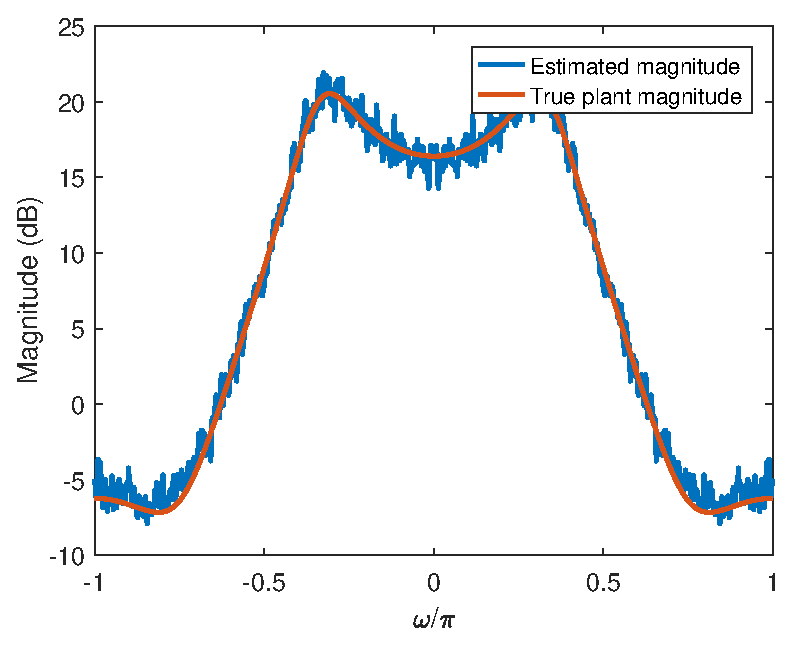
\includegraphics[width=\textwidth]{../homework/figs/inverse_control_kramers_kronig_id_mag.eps}
		\end{center}
	\end{column}

	\begin{column}{0.5\textwidth}
	\textbf{Phase:}	
	\begin{center}
		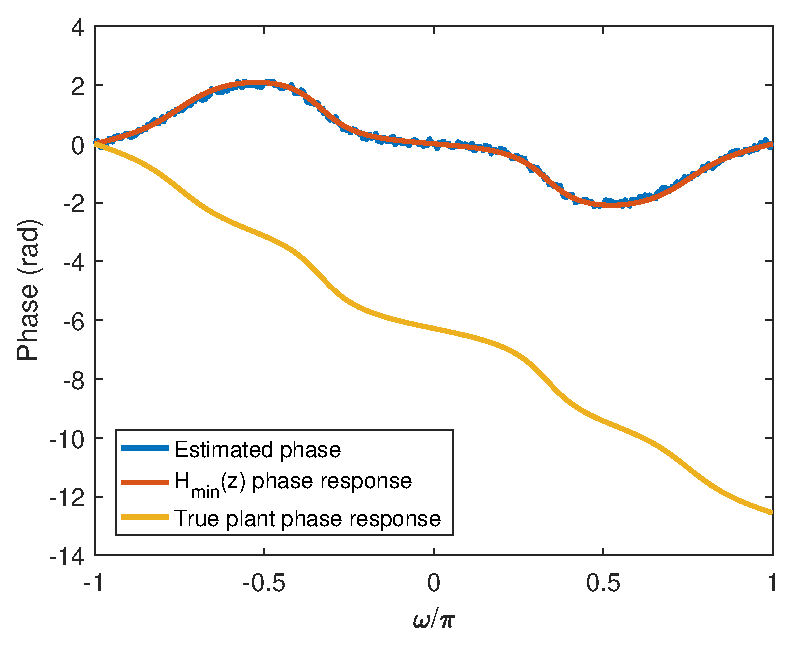
\includegraphics[width=\textwidth]{../homework/figs/inverse_control_kramers_kronig_id_phase.eps}
	\end{center}
	\end{column}
\end{columns}

As expected, we can only estimate the phase of the minimum phase system.
\end{frame}

%
\begin{frame}{Plant identification}
Applying the definition of cross-correlation:
\begin{align*}
\phi_{yx}[m] &= \E(y[m]\ast x^*[-m]) \\
&= \E(h[m]\ast x[n] \ast x^*[-m]) \tag{since $y[n] = h[n]\ast x[n]$} \\
& = h[m]\ast \E(x[n] \ast x^*[-m]) \tag{since $h[n]$ is deterministic} \\
& = h[m]\ast \phi_{xx}[m] \\
\end{align*}

If we have estimates for both $\phi_{yx}[m]$ and $\phi_{xx}[m]$ (easy using \texttt{xcorr}), we can compute
\begin{equation*}
H(e^{j\omega} = \frac{\Phi_{yx}(e^{j\omega})}{\Phi_{xx}(e^{j\omega})}
\end{equation*}

We know how to estimate $\Phi_{xx}(e^{j\omega})$ e.g., Welch's method, Blackman-Tukey method. But how do we estimate $\Phi_{yx}(e^{j\omega})$
\end{frame}



%
\begin{frame}{Modified Blackman-Tukey method}
\begin{enumerate}
	\item Estimate the cross-correlation function from $Q$ samples of $x[n]$ and $y[n]$
	\begin{equation*}
	\hat{\phi}_{yx}[m] = \frac{1}{Q-|m|}\sum_{n = 0}^{Q-1-|m|} y[m+n]x^*[n], \quad |m|\leq Q-1
	\end{equation*}
	\item Multiply cross-correlation by window $w[m]$
	\begin{equation*}
	s[m] = \begin{cases}
	\hat{\phi}_{yx}[m]w[m], & -(M-1)\leq m \leq (M-1) \\
	0, & \text{otherwise}
	\end{cases}
	\end{equation*}
	window is centered around $m = 0$ and it has length $L = 2M-1$.
	\item Compute DFT
	\begin{equation*}
	S[k] = \sum_{m = 0}^{N-1}s[m]e^{-j(2\pi/N)k}, \quad k = 0, \ldots, N-1
	\end{equation*}
	Because of the indexing of the DFT $S[k] = \hat{\Phi}_{yx}(e^{j(2\pi/N)k})e^{j(2\pi/N)M}$. We must remove the phase shift $e^{j(2\pi/N)M}$.
\end{enumerate}
\end{frame}

%
\begin{frame}{Modified Blackman-Tukey method}
Equivalent code:

\begin{align*}
&\texttt{phi\_yx\_hat = xcorr(y, x, M-1, 'unbiased')} \\
&\texttt{s = phi\_yx\_hat.*window} \\
&\texttt{S = fftshift(fft(ifftshift(s)))}
\end{align*}

Instead of correcting the phase shift $e^{j(2\pi/N)M}$ by multiplying \texttt{S} by $e^{-j(2\pi/N)M}$, we can use the command \texttt{ifftshift(s)} to correct the indexing.

\end{frame}
	
%
\begin{frame}{Plant identification}
This time we could also estimate the correct phase response.
	\begin{columns}
		\begin{column}{0.5\textwidth}
			\textbf{Magnitude:}	
			\begin{center}
				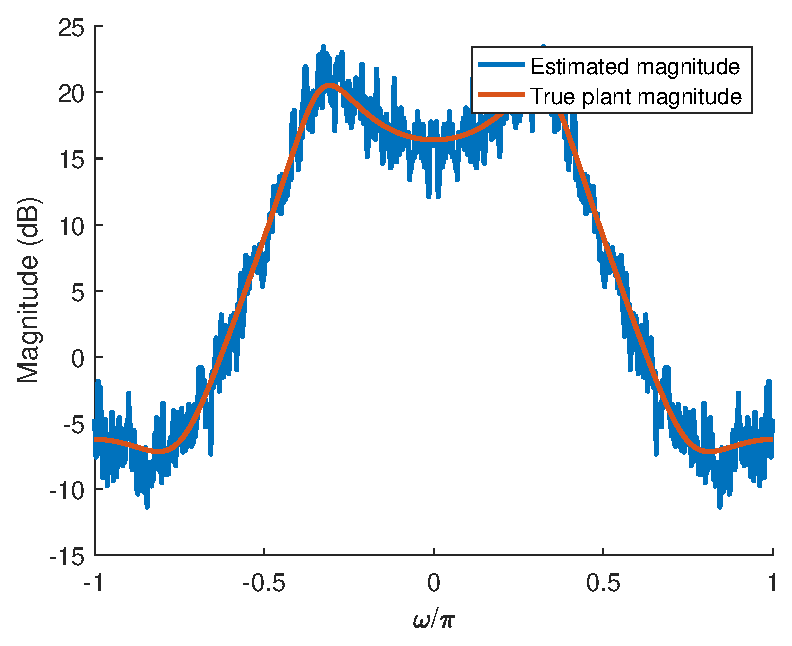
\includegraphics[width=\textwidth]{../homework/figs/inverse_control_xcorr_id_mag.eps}
			\end{center}
		\end{column}
		
		\begin{column}{0.5\textwidth}
			\textbf{Phase:}	
			\begin{center}
				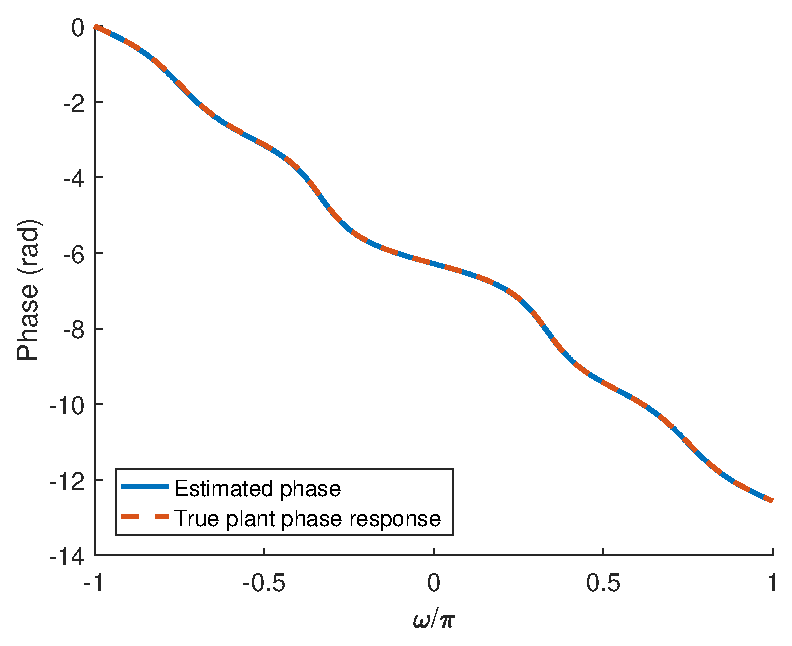
\includegraphics[width=\textwidth]{../homework/figs/inverse_control_xcorr_id_phase.eps}
			\end{center}
		\end{column}
	\end{columns}
\end{frame}

%
\begin{frame}{Controller design: linear phase FIR filter}
	The desired response is 
	\begin{equation*}
		H_d(e^{j\omega}) = H_{min}^{-1}(e^{-j\omega})
	\end{equation*}
	
	Since, $H_{min}^{-1}(e^{-j\omega})$ does not have any discontinuities, we can use $W(\omega) = 1~\forall\omega$.
	
	\begin{center}
		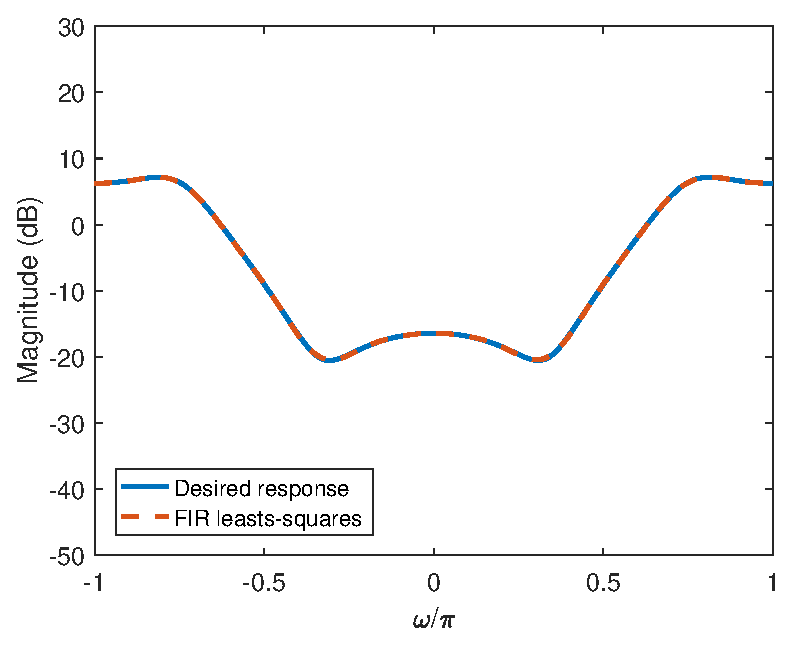
\includegraphics[width=0.6\textwidth]{../homework/figs/inverse_control_controller_linear_phase.eps}
	\end{center}
	
	Although, the magnitude is matched almost perfectly the minimum phase system does not have linear phase. 
\end{frame}

%
\begin{frame}{Controller design: non-linear phase FIR filter}
\begin{enumerate}
\item Calculate matrix $Q$, as usual
\item Calculate vector $d$ by sampling $H_d(e^{j\omega})$, as usual
\item $h = Q^{\dagger}d$.
\end{enumerate}

Make sure that $h$ is real. In numerical computations, the imaginary part of $h$ will be small. Hence, we can discard the imaginary part
\begin{equation*}
	\texttt{>> hls = real(pinv(Q)*d)}
\end{equation*}

\begin{columns}
	\begin{column}{0.45\textwidth}
		\textbf{Magnitude:}	
		\begin{center}
			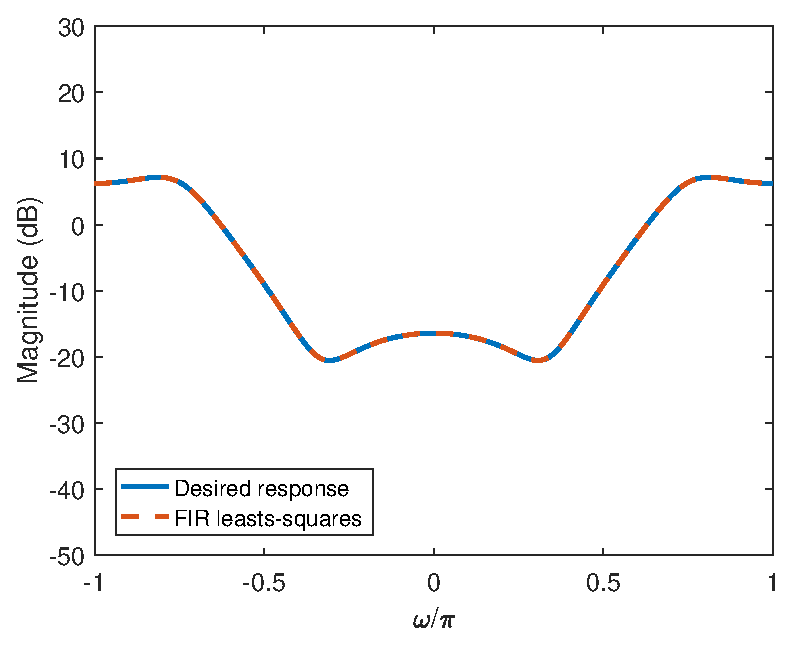
\includegraphics[width=\textwidth]{../homework/figs/inverse_control_controller_nonlinear_phase_mag.eps}
		\end{center}
	\end{column}
	
	\begin{column}{0.45\textwidth}
		\textbf{Phase:}	
		\begin{center}
			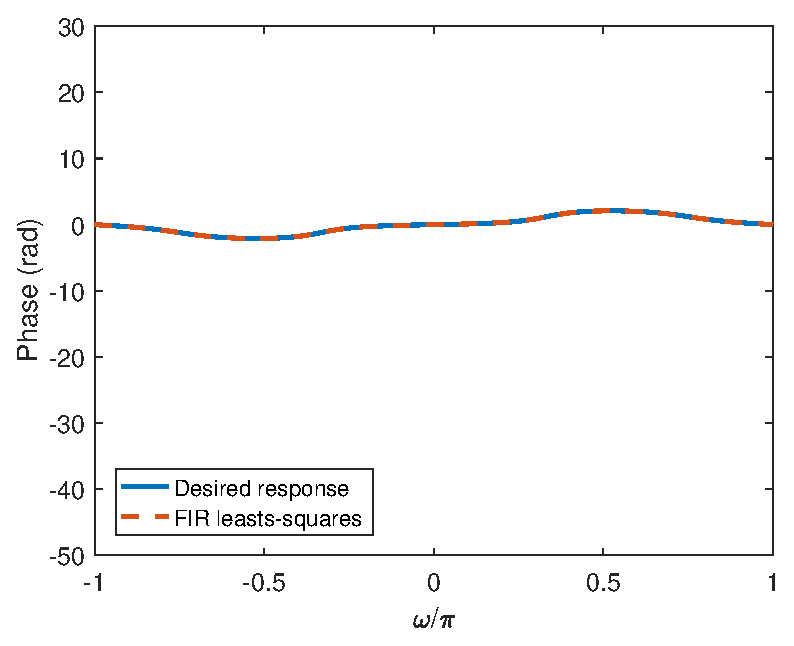
\includegraphics[width=\textwidth]{../homework/figs/inverse_control_controller_nonlinear_phase_phase.eps}
		\end{center}
	\end{column}
\end{columns}

This will be a good controller because it matches both the magnitude and phase of the desired response.

\end{frame}

%
\begin{frame}{Testing the controller}
\begin{center}
	\resizebox{0.7\textwidth}{!}{\begin{tikzpicture}[->, >=stealth, shorten >= 0pt, draw=black!50, node distance=3.2cm, font=\sffamily]
    \tikzstyle{node}=[circle,fill=black,minimum size=2pt,inner sep=0pt]
    \tikzstyle{block}=[draw=black,rectangle,fill=none,minimum size=1.5cm, inner sep=0pt]

	\node[node] (xc) {};
    \node[block, right=1cm of xc] (C) {$C(z)$};
    \node[block, right of=C] (P) {$H(z)$};
	\coordinate[right=1cm of P] (yc) {};
	
	\coordinate (mid1) at ($(P.east)!0.5!(C.west)$) {};
		
    \path (xc) edge (C);
    \path (C) edge (P);
    \path (P) edge (yc);
    
    \node[above = 0.5mm of mid1] {$x[n]$};
    \node[above = 0mm of xc, text width = 1cm, align=center] {$s[n]$};
    \node[above = 0mm of yc, text width = 1cm, align=center] {$y[n]$}; 
    \node[below] at ($(C.south)$) {Controller};
    \node[below] at ($(P.south)$) {Plant};
\end{tikzpicture}}
\end{center}

The input $s[n]$ will be:
\begin{description}
	\item[(a)] Unit step. 
	\item[(b)] Sinusoid of frequency $0.1\pi$.
	\item[(b)] Sinusoid of frequency $0.9\pi$. 
\end{description}

\end{frame}


%
\begin{frame}{Testing the controller: unit step}
The plant does not respond immediately to the command.
\begin{center}
	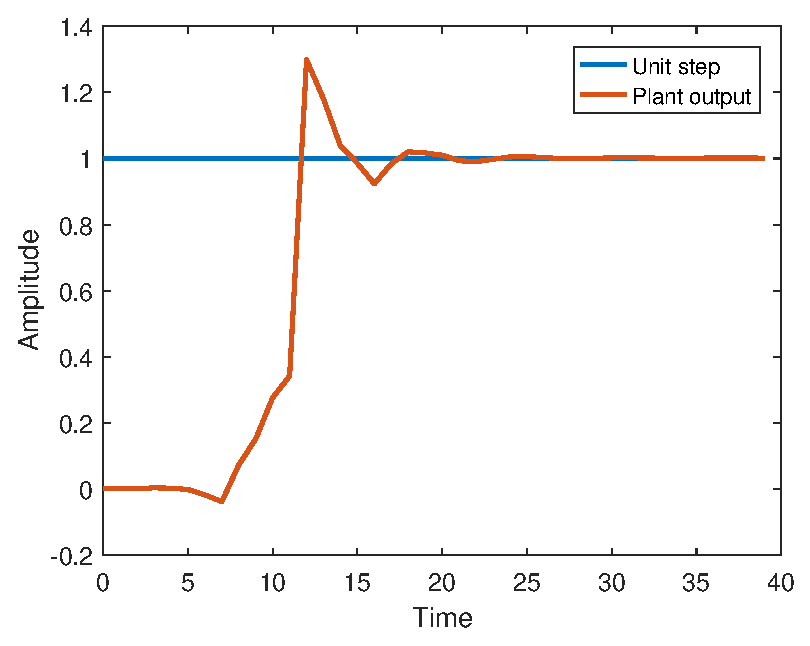
\includegraphics[width=0.8\textwidth]{../homework/figs/inverse_control_unit_step.eps}
\end{center}
\end{frame}

%
\begin{frame}{Testing the controller: sinusoid input}
Input is $s[n] = \sin(0.1\pi n)$
\begin{center}
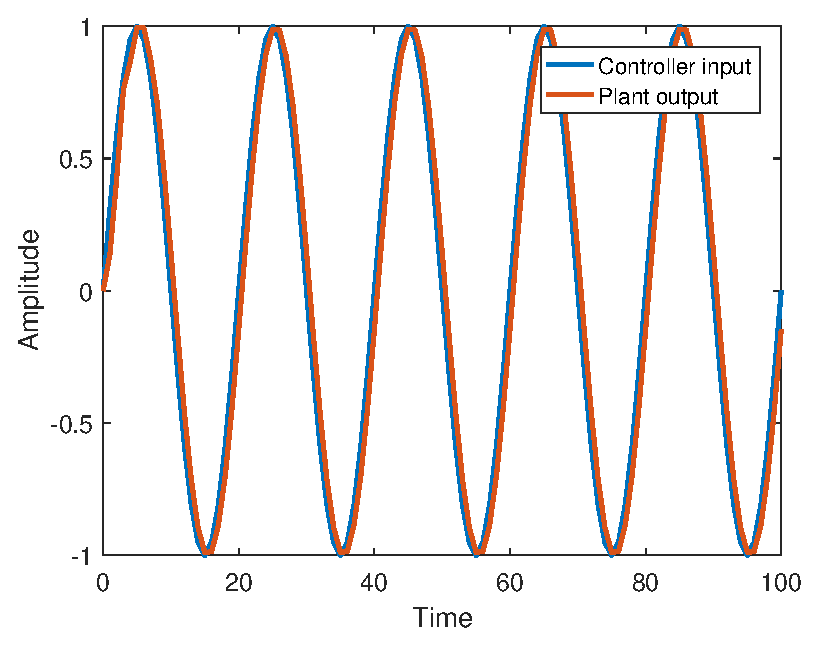
\includegraphics[width=0.8\textwidth]{../homework/figs/inverse_control_sin1.eps}
\end{center}

Group delay of controller + plant is small at $\omega = 0.1\pi$.
\end{frame}

%
\begin{frame}{Testing the controller: sinusoid input}
Input is $s[n] = \sin(0.9\pi n)$
\begin{center}
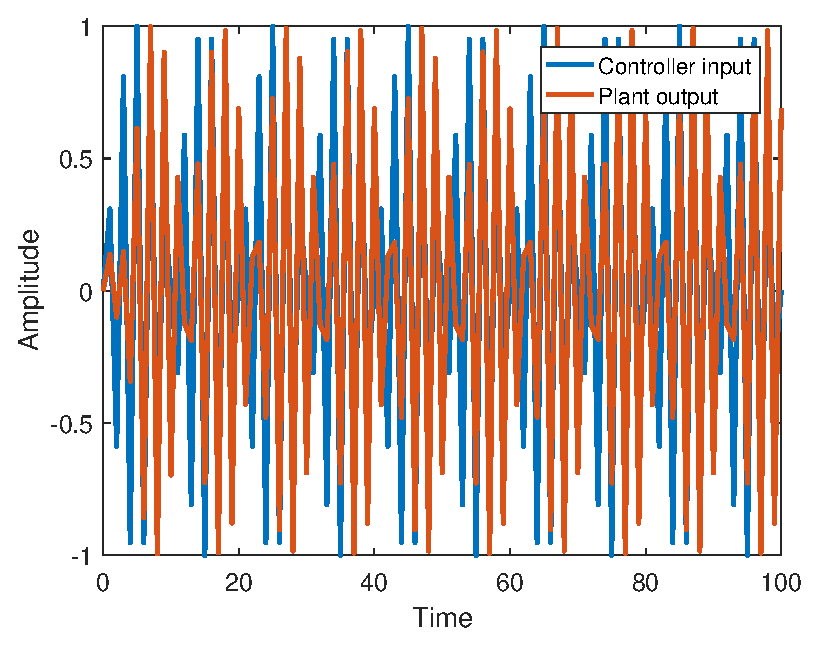
\includegraphics[width=0.8\textwidth]{../homework/figs/inverse_control_sin2.eps}
\end{center}

Group delay of controller + plant is noticeable at $\omega = 0.9\pi$.
\end{frame}

%
\begin{frame}{What's next?}
There's a lot more to learn
\begin{itemize}
\item EE 373A: Adaptive signal processing
\item EE 278: Introduction to statistical signal processing
\item EE 378A: Statistical signal processing
\item EE 378B: Inference, estimation, and information processing
\item EE 368: Image signal processing	
\end{itemize}
\end{frame}



\end{document}
